\documentclass[11pt, oneside]{article}   	% use "amsart" instead of "article" for AMSLaTeX format
\usepackage{geometry}                		% See geometry.pdf to learn the layout options. There are lots.
\geometry{letterpaper}                   		% ... or a4paper or a5paper or ... 
%\geometry{landscape}                		% Activate for for rotated page geometry
%\usepackage[parfill]{parskip}    		% Activate to begin paragraphs with an empty line rather than an indent
\usepackage{graphicx}				% Use pdf, png, jpg, or eps� with pdflatex; use eps in DVI mode
								% TeX will automatically convert eps --> pdf in pdflatex		
\usepackage{amssymb}
\usepackage{amsmath}
\usepackage{parskip}
\usepackage{color}

\title{Triple Integrals - Intro}
%\author{The Author}
%\section{}
% \subsection*{R code}
\date{}							% Activate to display a given date or no date

\graphicspath{{/Users/telliott_admin/Dropbox/Tex/png/}}

% \begin{bmatrix} a  &  b \\ c  &  d \end{bmatrix}
% \bigg |_

\begin{document}
\maketitle
\Large

For double integrals, we have a function $f(x,y)$, although for a simple area this function might be 1, and we think of the value of the function at each point $(x,y)$ over a region $R$ as a height in the $z$-dimension.  So for the double integral what we visualize is a surface in three dimensions, and  we are computing the volume underneath the surface over the region $R$ that is its shadow of this in the $xy$-plane.

We do that by taking slices through this volume that are perpendicular to one of the axes, say the $x$-axis, and each of this series of thin slices has a volume which is an area times a thickness that is $dx$.  The area calculation is a standard 1D integral of the slice across the range of $y$.  The biggest trick is to remember that the limits for $y$ in the inner integral usually depend on which slice we are talking about (i.e. the current value of $x$).  The bounds of $R$, the limits for $y$, often depend on where we are along the x-axis.  The outer integral always goes from the smallest to largest values of $R$ in that dimension.

For a triple integral, we can no longer visualize the thing we are computing as a volume, unless you are able to visualize it as a volume in four dimensions.  Instead we have two things:  a function which associates with a value with every point in 3D space inside some solid, and in conjunction a description of this solid or volume which is the 3D analog of the region $R$ that was the shadow of our surface for a double integral.

Remember that in double integrals it was the shape of the region that determined the bounds on the integrals.  It will be similar for triple integrals, but harder to visualize.

%\noindent
Strang starts this topic with a box, and you can't get simpler than that.  Suppose it is $[0,2] \times [0,3] \times [0,1]$.
\[ V = \iiint  dV = \int_{z=0}^1 \int_{y=0}^3 \int_{x=0}^2 dx \ dy \ dz \]
\[ = \int_{z=0}^1 \int_{y=0}^3 x \bigg |_0^2 \ dy \ dz \]
\[ = 2 \int_{z=0}^1 y \bigg |_0^3 \ dz \]
\[ = 6 \int_{z=0}^1 dz = 6 \]
What about half a box?  Call it a doorstop or \emph{prism}.  We can slice the object in various ways.  
\begin{center} 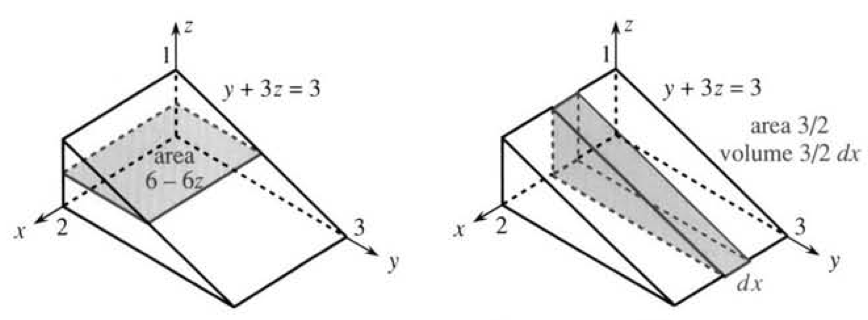
\includegraphics [scale=0.4] {wedge.png} \end{center}
For the approach in the left panel, we have slices of area added up as we go along the $z$-axis.  
The question is, what are the bounds if the outer integral is of $dz$ with $z=0 \rightarrow z = 1$.  If we do $dx$ as the middle one, notice that $x$ does not depend on $z$ so the bounds are $x=0 \rightarrow x=2$.  The only variable bounds are on $y$.  $y$ depends on $z$, and the equation for the outer bound is $y=3-3z$.  So this integral is
\[  \int_{z=0}^1 \int_{x=0}^2 \int_{y=0}^{3-3z}  dy \ dx \ dz \]
\[  \int_{z=0}^1 \int_{x=0}^2 3-3z \ dx \ dz \]
\[  \int_{z=0}^1 (3-3z)x \bigg |_0^2 \ dz \]
\[  \int_{z=0}^1 6-6z \ dz = 6z - 3z^2 \bigg |_0^1 = 3 \]
For the approach in the right panel, our slices of area are parallel to the $yz$-plane.  We have the same equation ($y=3-3z$), but solve this time for $z$.
\[  \int_{x=0}^2 \int_{y=0}^3 \int_{z=0}^{1-\frac{1}{3} y}  dz \ dy \ dx \]
\[  \int_{x=0}^2 \int_{y=0}^3 1-\frac{1}{3} y  \ dy \ dx \]
\[  \int_{x=0}^2  y-\frac{1}{6} y^2  \bigg |_0^3 \ dx \]
\[  \int_{x=0}^2  \frac{3}{2}  \ dx = 3 \]
\subsection*{cone}
The hard part about the cone is simply coming up with the right volume element for cylindrical coordinates
\[ V = \iiint dz \ r \ dr \ d \theta \]
which can be seen if we remember that a small change in $\Delta \theta$ gives a small change in length on the surface of $r \Delta \theta$.  And of course we can check it for the cylinder with radius $r=2$ and height $h=2$
\[ V = \int_0^{2 \pi} \int_0^r \int_0^2 dz \ r \ dr \ d \theta \]
\[ = 2 \ \int_0^{2 \pi} \int_0^r \ r \ dr \ d \theta \]
\[ = 4 \pi \ (\frac{1}{2} r^2 \ \bigg |_0^2 ) = 8 \pi \]
\[ V = \iiint dz \ r \ dr \ d \theta \]
For a cone with height $h=1$ and radius $r=1$, if we fix $r$, what are the bounds on $z$?  $z$ ranges from $0 \rightarrow 1-r$.
\[ V = \int_0^{2 \pi} \int_0^1 \int_0^{1-r} dz \ r \ dr \ d \theta \]
\[ = \int_0^{2 \pi} \int_0^1 (1-r) \ r \ dr \ d \theta \]
\[ = \int_0^{2 \pi} \frac{1}{2}r^2 - \frac{1}{3}r^3 \ \bigg |_0^1 \ d \theta \]
\[ 2 \pi \ \frac{1}{6} = \frac{\pi}{3} \]

For a general cone, an important thing is that the ratio of $R/H$ is fixed so that at any height $h$
\[ r = \frac{R}{H} h \]
\[ h = \frac{H}{R} r \]
So again, given fixed $r$ (and $\theta$), what are the bounds on $z$?  They are $0 \rightarrow  H - \frac{H}{R}r$.
\[ V = \int_0^{2 \pi} \int_0^R \int_0^{H- \frac{H}{R}r} dz \ r \ dr \ d \theta \]
\[ V = \int_0^{2 \pi} \int_0^R (H - \frac{H}{R}  r) \ r \ dr \ d \theta \]
\[ V = \int_0^{2 \pi} \frac{1}{2} H R^2 - \frac{1}{3} \frac{H}{R}  R^3 \ d \theta \]
\[ V = \int_0^{2 \pi} \frac{1}{6} H R^2 \ d \theta \]
\[ V = \frac{1}{3} \pi \ HR^2 \]

\subsection*{tetrahedron}
\begin{center} 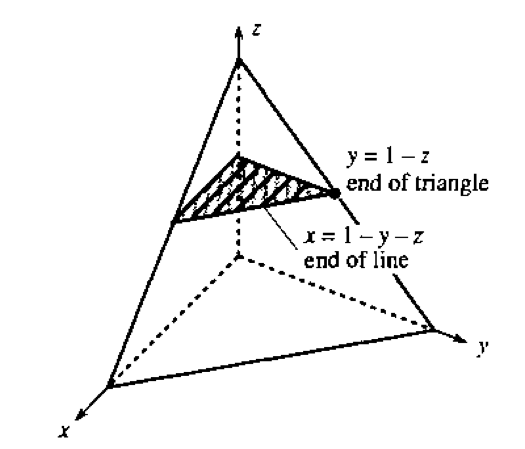
\includegraphics [scale=0.4] {tetrahedron.png} \end{center}
We have a tetrahedron with one vertex at the origin and the other $3$ on the axes, $1$ unit away from the origin.  Suppose we slice horizontally, adding up slices as we move along $z = 0 \rightarrow 1$.  As the figure shows, the lines that we will sum up to give each slice of area are in the $x$ direction.  So our integral looks like
\[  \iiint dx \ dy \ dz \]
We need to find the bounds for $x$ and $y$.  We do $y$ first.  In the $yz$-plane, the dependence of $y$ on $z$ is $y + z = 1$ or $y = 1 - z$.
\[ V =  \int_{z=0}^1 \int_{y=0}^{1-z} \int  dx \ dy \ dz \]
What about $x$?  Notice that the equation of the plane is
\[ x + y + z = 1 \]
So $x = 1 - y - z$ and
\[ V =  \int_{z=0}^1 \int_{y=0}^{1-z} \int_{x=0}^{1-y-z}  \ dx \ dy \ dz \]
\[ =  \int_{z=0}^1 \int_{y=0}^{1-z} 1-y-z \  dy \ dz \]
\[ =  \int_{z=0}^1 y- \frac{1}{2}y^2 - yz  \bigg |_0^{1-z} \ dz \]
\[ =  \int_{z=0}^1 1 - z - \frac{1}{2}(1-z)^2 - (1-z) z \ dz \]
\[ =  \int_{z=0}^1 1 - z - (1-z) z - \frac{1}{2}(1-z)^2 \ dz \]
\[ =  \int_{z=0}^1 (1 - z)^2 - \frac{1}{2}(1-z)^2 \ dz \]
\[ =  \int_{z=0}^1 \frac{1}{2}(1 - z)^2    \ dz  \]
\[ =  -\frac{1}{2}\frac{1}{3}(1 - z)^3 \bigg |_0^1 = \frac{1}{6}  \]

(Faster), notice that for each slice $x=y$ so we could do
\[ V =  \int_{z=0}^1 \int_{y=0}^{1-z} \int_{x=0}^{y}  \ dx \ dy \ dz \]
\[ V =  \int_{z=0}^1 \int_{y=0}^{1-z} y \ dy \ dz \]
\[ V =  \int_{z=0}^1 \frac{1}{2}(1-z)^2 \ dz \]
and so on.

Looking again at the figure
\begin{center} 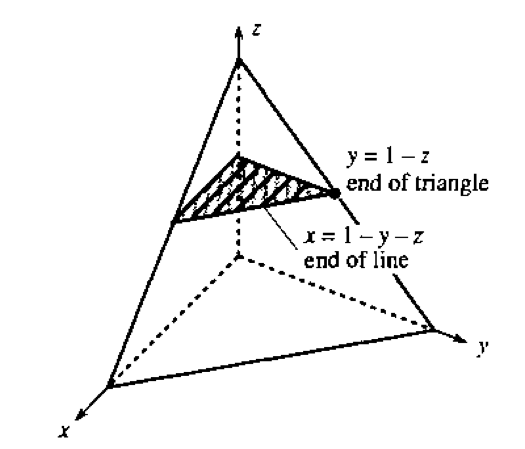
\includegraphics [scale=0.4] {tetrahedron.png} \end{center}
The area of the base is $\frac{1}{2}$ (half the unit square), the height is $1$, and there is the extra factor of $\frac{1}{3}$ for the volume of a pyramid.

A more laborious calculation is that the length of each edge is $\sqrt{2}$, the length of the altitude of any face is 
\[ h = \sqrt{2} \frac{\sqrt{3}}{2} \]
The area of the face is then
\[ \frac{1}{2} \ base \times height = \frac{1}{2} \sqrt{2} \sqrt{2} \frac{\sqrt{3}}{2} = \frac{\sqrt{3}}{2} \]
To get the correct volume, the coordinates of the point in the plane closest to the origin must be
\[ P = (\frac{1}{3},\frac{1}{3},\frac{1}{3}) \]
(by symmetry, and because $x+y+z=1$), 
and the distance from the origin is then
\[ d = \sqrt{(\frac{1}{3})^2 + (\frac{1}{3})^2 + (\frac{1}{3})^2 } = \frac{1}{\sqrt{3}} \]
and the volume is
\[ V = \frac{1}{3} \ area \times height = \frac{1}{3} \ \frac{\sqrt{3}}{2} \  \frac{1}{\sqrt{3}} = \frac{1}{6}  \] 
as we expected.
\subsection*{center of mass}
Naturally, we do not need such a fancy method to find the volumes of regular solids, nor even for an ellipsoid.  However, if we have some other quantity that varies with position like density = $\rho(x,y,z)$, then we just integrate with that too.  For example, let's find the average height of $z$, called $\bar{z}$.  (The centroid is at $\bar{x},\bar{y},\bar{z}$).
 
\[ \iiint  z dV = \int_{z=0}^1 \int_{y=0}^{1-z} \int_{x=0}^{x=y}  z \ dx \ dy \ dz \]
\[ = \int_{z=0}^1 \frac{1}{2} z(1-z)^2 \ dz \]
\[ = \int_{z=0}^1 \frac{1}{2}z - z^2 + \frac{1}{2}z^3 \ dz \]
\[ = \frac{1}{4}z^2 - \frac{1}{3}z^3 + \frac{1}{8}z^4 \bigg |_0^1 = \frac{1}{24} \]
\[ \bar{z} = \frac{ \iiint z \ dV}{\iiint dV} = \frac{1}{24} / \frac{1}{6} = \frac{1}{4} \]

\subsection*{Auroux}

His first example considers the shape constructed from two surfaces, one above $z = x^2 + y^2$ and the second underneath $z = 4 - x^2 - y^2$.  These are both paraboloid surfaces, and they have a plane of symmetry at $z = 2$.  We consider the function $1$, that is, we want to compute the volume of this solid.

(Incidentally, we know the answer to this problem already.  If we turn the paraboloid on its side, and put the vertex at the origin, then we will have the curve $y=\sqrt{x}$.  Calculate its volume as a solid of revolution as $\int \pi y^2 \ dx = \pi \int x \ dx = \pi/2 \ x^2$.  We obtain $2\pi$ with the limits $x=0 \rightarrow x=2$, this is for each symmetric half of the solid, or $4\pi$ total.

So we want to set up the triple integral
\[ \iiint dV \]
and the question is, what are the bounds?  The solid has vertical mirror image symmetry, and the place where the two functions are equal is
\[  4 - x^2 - y^2 = x^2 + y^2 \]
\[  2 = x^2 + y^2 \]

The easiest way to do this is to integrate first with respect to $z$, since we know that $z$ goes from $x^2 - y^2 \to 4 - x^2 + y^2$.  Imagine that we have a dipstick that goes through the engine, it only gets wet in the middle, and the bounds of the wet part are as above.  So then the question is, for each value of $z$ that is contained in our solid, what are $x$ and $y$?

The trick here is that the other bounds are for the circle $x^2 + y^2 = 2$, this is the largest cross-section of our solid.  So Auroux sets up this integral

\[ \int_{x=-\sqrt{2}}^{x=\sqrt{2}} \int_{y=-\sqrt{2-x^2}}^{y=\sqrt{2-x^2}} \int_{z=x^2 + y^2}^{z=4- x^2 - y^2} dz \ dy \ dx \]

Notice that these $xy$-bounds go over the entire region, that is the shadow of the solid in the xy-plane.  This is a little counterintuitive to me, given how careful we were in double integrals about the bounds start and stop, but it's because that is all taken care of by the $z$ term.  We integrate over the whole disk and in the inside we let z go between the appropriate bounds.

He goes on to set up the integral in cylindrical coordinates.  The inner integral is the same, but the outer integrals are changed to polar coordinates (and in particular, $x^2 + y^2 = r^2$

\[ \int_{\theta =0}^{\theta=2\pi} \int_{r=0}^{r=\sqrt{2}} \int_{z=r^2}^{z=4- r^2} dz \ r \ dr \ d\theta \]
The inner integral is:
\[ \int_{z=r^2}^{z=4 - r^2} dz  \]
\[ = 4 - 2r^2 \]
The middle integral is then
\[ \int_{r=0}^{r=\sqrt{2}} (4 - 2r^2) \ r \ dr  \]
\[ = 2r^2 - \frac{1}{2}r^4 \ \bigg |_0^{\sqrt{2}} = 4 - 2 = 2 \]
And the outer integral is just
\[ \int_{\theta =0}^{\theta=2\pi} 2 \ d\theta = 4 \pi \]

\end{document}  